\chapter*{Podsumowanie}
\addcontentsline{toc}{chapter}{Podsumowanie}
\section*{Podsumowanie projektu}
\addcontentsline{toc}{section}{Podsumowanie projektu}
Przedstawiona w niniejszej pracy realizacja języka TQL spełnia najważniejsze postulaty. 
Po pierwsze jest on intuicyjny i prosty w użyciu dla osób znających jedynie dziedzinę problemu.
% (co potwierdza opinia dr hab. Marka Stępnia)
Po drugie minimalnie ogranicza siłę wyrazu, pozwalając na tworzenie skomplikowanych zapytań.

%TODO: to jest trochę podobne do tego, co piszę w dyskusji
Język TQL ma jednak kilka ograniczeń w stosunku do typowych języków zapytań. 
Największym z nich jest brak wpływu na postać wyniku, co utrudnia np. zbieranie danych statystycznych 
(m.in. nie da się spytać o ilość tabliczek spełniających dane kryteria). 
Można jednak stworzyć narzędzia do samej prezentacji wyników zapytań, które pokonają to ograniczenie. 

Należy pamiętać, że TQL jest jedynie językiem wyszukiwania -- w przeciwieństwie do wielu innych języków zapytań
nie udostępnia możliwości zmieniania danych znajdujących się w bazie, ani dodawania nowych. 

%zalety
Dzięki specyficznym cechom języka TQL, można również dostosować go do wykorzystania w innych dziedzinach. 
Należy tu wspomnieć o braku ograniczenia ilości i nazw pól, po których można wyszukiwać, oraz przystosowaniu 
do wyszukiwania wg kryteriów dotyczących danych tekstowych. 
Na podstawie TQL można łatwo stworzyć rodzinę języków dla różnych dziedzin zajmujących się przeszukiwaniem tekstów.

%luźne uwagi
W ramach niniejszej pracy zaprezentowane zostały dwie implementacje języka TQL. 
Po stworzeniu pierwszej, czas potrzebny na drugą był już niewielki. 
Największym zadaniem było przetłumaczenie poszczególnych konstrukcji TQL na XQuery. 
Pozwala to sądzić, że każda kolejna implementacja, dla różnych typów baz i różnych schematów danych, 
nie będzie wymagała dużego nakładu pracy. 

\newpage 

\section*{Możliwości rozwoju}
\addcontentsline{toc}{section}{Możliwości rozwoju}
\begin{figure}[h]
 \centering
 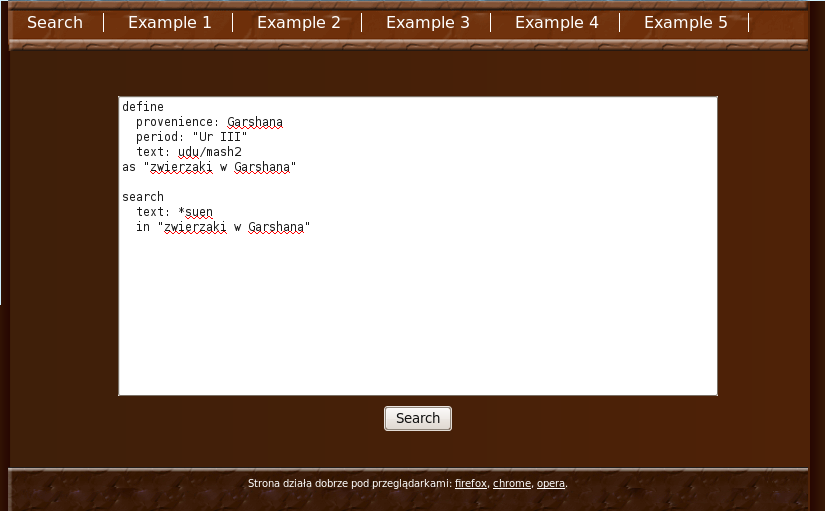
\includegraphics[width=450px]{../diagramy/wyszuk_zapyt.png}
 % wyszuk_zapyt.png: 811x524 pixel, 72dpi, 28.61x18.49 cm, bb=0 0 811 524
 \caption{Okno do wprowadzania zapytania}
 \label{fig:wyszuk_zapyt}
\end{figure}

\begin{figure}[h]
 \centering
 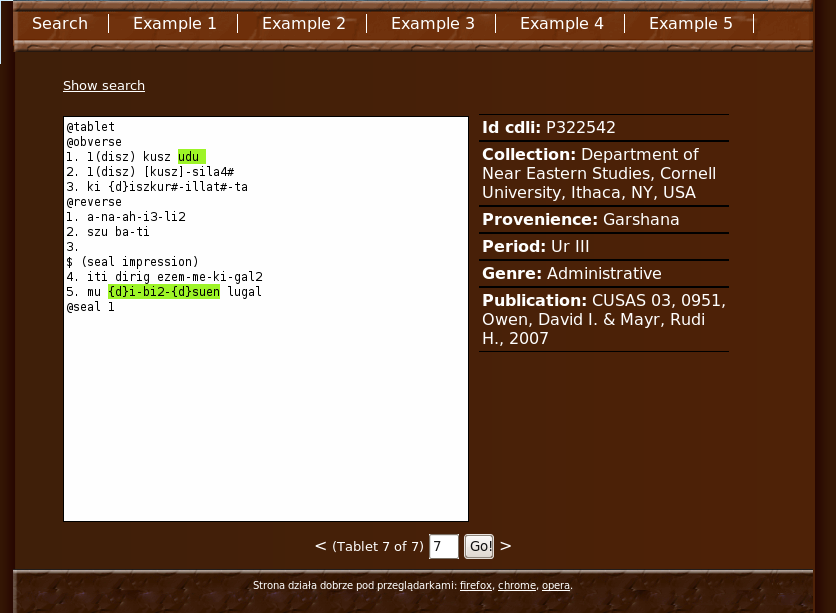
\includegraphics[width=450px]{../diagramy/wyszuk_wynik.png}
 % wyszuk_wynik.png: 823x628 pixel, 72dpi, 29.03x22.15 cm, bb=0 0 823 628
 \caption{Sposób prezentacji wyników zapytania}
 \label{fig:wyszuk_wynik}
\end{figure}

%co dalej
Jako dodatek do pracy stworzyłyśmy stronę internetową umożliwiającą zadanie zapytania w języku TQL i prezentującą wyniki. 
Jej wygląd jest przedstawiony na rysunkach \ref{fig:wyszuk_zapyt} oraz \ref{fig:wyszuk_wynik}.
% TODO: W chwili obecnej jest ona dostępna na stronie \url{http://students.mimuw.edu.pl/~/jw234694/sumlib/}.
Stanowi ona zalążek przyjaznego interfejsu użytkownika dla naukowców, którzy będą współpracować z TQL. Plany jej rozwoju
uwzględniają między innymi funkcjonalność graficznego budowanie zapytania.
% TODO: walnąć rozdzialik o graficznym bilderze
Na chwilę obecną serwis internetowy jest w trakcie udostępniania Wydziałowi Historii UW.
Jego pracownicy będą pierwszymi testerami całego rozwiązania.

Poza tym warto nawiązać współpracę z projektem CDLI, (zob. rozdział \ref{chapter:cdli}).
Implementacja TQL dla bazy CDLI, wraz z interfejsem www, z pewnością byłaby przydatnym narzędziem dla sumerologów na całym świecie.

W dalszej perspektywie można rozwinąć język TQL między innymi o wyszukiwanie wg klinów i wg tagów. 
Pierwsze z nich wymaga przetłumaczenia odczytów na kliny oraz umieszczenia tych informacji w bazie danych.
Drugie natomiast potrzebuje narzędzia do wykrywania poszczególnych tagów
(postaci, miar, dat, liczb itp) lub do ich zaznaczania przez sumerologów.

Dodatkowo warto stworzyć narzędzie do analizy uszkodzonych fragmentów i wykrywania błędów w odczytach tekstów. 
Dzięki niemu można by zmniejszyć ryzyko pominięcia istotnych tabliczek podczas wyszukiwania. 

Rozwój projektu będzie zależał również od potrzeb zgłaszanych przez samych sumerologów.


\section*{Dyskusja}
\addcontentsline{toc}{section}{Dyskusja}
% co można by inaczej (``Dyskusje'')

% konstrukcja języka
%zapytanie, którego się nie da wyrazić
Język TQL pozwala wyrazić wiele zapytań w prosty sposób, ale istnieją również takie, których nie da się w nim zapisać.
Przykładem takiego zapytania jest "znajdź tabliczki, które zawierają frazę zaczynającą się od słowa udu, której drugim słowem nie jest słowo ban".
Ogólnie TQL pozwala tworzyć zapytania w oparciu o frazy, określone w całości lub częściowo, ale nie pozwala konstruować warunków
dotyczących fragmentów fraz. Godzimy się na to ograniczenie, ponieważ najczęściej nie jest to potrzebne. Niemniej jednak
warto rozważyć alternatywną konstrukcję języka, która umożliwi zapisywanie tego typu zapytań.

%sortowanie
Warto również zastanowić się nad możliwością sortowania wyników zapytań. W obecnej wersji TQL moża to zrobić na poziomie interfejsu, jednak
dodanie takiej funkcjonalności do języka pozwoliłoby na sortowanie bezpośrednio w bazie danych.

% implementacja
Przedstawiona w pracy implementacja TQL jest tylko przykładowa. W szczególności można rozważyć optymalizacje w modułach zależnych od bazy
danych, czyli wybór takiego sposobu budowania zapytania docelowego, który pozwoli jak najszybciej je wykonać. 
% c++, LL, Boost spirit
% wymyśleć inne zapytanie na ``NOT''
W tym momencie implementacja zapytania zawierającego "-- --" (not) jest dla bazy PostgreSQL nieoptymalna.
Polega ona na wyszukaniu wszystkich tabliczek, następnie wyszukaniu tabliczek zawierających niechcianą frazę, a potem odjęciu obu wyników.
Można tutaj zaproponować algorytm, który będzie działał szybciej.

% co jest złego w typowej relacyjnej bazie danych
Innym problemem, który również warto rozważyć przy implementacji TQL, jest wybór odpowiedniego sposobu reprezentacji danych. Szeroko rozpowszechnione
bazy relacyjne nie są najlepszym rozwiązaniem, gdyż trudno w nich przeprowadzać operacje na tekstach. Potrzebna jest baza, która umożliwi jednocześnie szybki
dostęp do całego tekstu, jak również szybkie wyszukiwanie fraz. Pomysł przedstawienia treści tabliczki za pomocą grafu pozwala na łatwe wyszukiwanie fraz oraz
alternatywnych tłumaczeń, jednak bazy relacyjne nie są przystosowane do przechowywania takich struktur danych.

% przenośność między systemami operacyjnymi

